\begin{filecontents*}[overwrite]{references.bib}
% Verified 2026-11-04 against Crossref, arXiv, NeurIPS proceedings metadata and publisher pages.
@techreport{shehabi2024lbnl,
  author      = {Shehabi, Arman and Smith, Sarah Josephine and Hubbard, Alex and Newkirk, Alexander and Lei, Nuoa and Siddik, Md AbuBakar and Holecek, Billie and Koomey, Jonathan G. and Masanet, Eric R. and Sartor, Dale A.},
  title       = {2024 United States Data Center Energy Usage Report},
  institution = {Lawrence Berkeley National Laboratory},
  address     = {Berkeley, CA, USA},
  number      = {LBNL-2001637},
  month       = dec,
  year        = {2024},
  doi         = {10.71468/P1WC7Q}
}
@techreport{iea2025energyai,
  author      = {{International Energy Agency}},
  title       = {Energy and {AI}},
  institution = {IEA},
  address     = {Paris, France},
  type        = {World Energy Outlook Special Report},
  month       = apr,
  year        = {2025},
  url         = {https://www.iea.org/reports/energy-and-ai}
}
@techreport{epri2026powering,
  author      = {Wilson, Thomas F. and Blanford, Geoffrey J. and Bistline, John and Johnson, Nils},
  title       = {Powering Intelligence 2026: Updated Scenarios of {U.S.} Data Center Electricity Use and Power Strategies},
  institution = {Electric Power Research Institute},
  address     = {Palo Alto, CA, USA},
  number      = {3002034696},
  month       = feb,
  year        = {2026}
}
@techreport{esig2025largeloads,
  author      = {{Energy Systems Integration Group}},
  title       = {Forecasting for Large Loads: Current Practices and Recommendations},
  institution = {Energy Systems Integration Group, Large Loads Task Force},
  address     = {Reston, VA, USA},
  month       = dec,
  year        = {2025},
  url         = {https://www.esig.energy/large-loads-task-force/forecasting/}
}
@article{shekhar2026review,
  author  = {Shekhar, Shivanshu and Tripathi, Shivanshu and Chawda, Gajendra Singh and Chaturvedi, Shivam and Su, Wencong and Wang, Mengqi and Ndoye, Mandoye and Oni, Ben},
  title   = {Critical Review of Artificial Intelligence and Machine Learning Methods for Data-Center Load Forecasting},
  journal = {Energies},
  volume  = {19},
  number  = {15},
  pages   = {3624},
  year    = {2026},
  doi     = {10.3390/en19153624}
}
@article{habib2026bridging,
  author  = {Habib, Md. Ahasan and Hossain, M. J. and Sakib, Sadnan and Alam, Md. Morshed},
  title   = {Bridging prediction and decision: An application-driven review of load forecasting in energy systems},
  journal = {Computers and Electrical Engineering},
  volume  = {134},
  pages   = {111113},
  year    = {2026},
  doi     = {10.1016/j.compeleceng.2026.111113}
}
@inproceedings{samsi2021supercloud,
  author    = {Samsi, Siddharth and Weiss, Matthew L. and Bestor, David and Li, Baolin and Jones, Michael and Reuther, Albert and Edelman, Daniel and Arcand, William and Byun, Chansup and Holodnack, John and Hubbell, Matthew and Kepner, Jeremy and Klein, Anna and McDonald, Joseph and Michaleas, Adam and Michaleas, Peter and Milechin, Lauren and Mullen, Julia and Yee, Charles and Price, Benjamin and Prout, Andrew and Rosa, Antonio and Vanterpool, Allan and McEvoy, Lindsey and Cheng, Anson and Tiwari, Devesh and Gadepally, Vijay},
  title     = {The {MIT} Supercloud Dataset},
  booktitle = {Proc. IEEE High Performance Extreme Computing Conference (HPEC)},
  pages     = {1--8},
  year      = {2021},
  doi       = {10.1109/HPEC49654.2021.9622850}
}
@article{koenker1978,
  author  = {Koenker, Roger and Bassett, Gilbert},
  title   = {Regression Quantiles},
  journal = {Econometrica},
  volume  = {46},
  number  = {1},
  pages   = {33--50},
  year    = {1978},
  doi     = {10.2307/1913643}
}
@article{gneiting2007,
  author  = {Gneiting, Tilmann and Raftery, Adrian E.},
  title   = {Strictly Proper Scoring Rules, Prediction, and Estimation},
  journal = {Journal of the American Statistical Association},
  volume  = {102},
  number  = {477},
  pages   = {359--378},
  year    = {2007},
  doi     = {10.1198/016214506000001437}
}
@inproceedings{ke2017lightgbm,
  author    = {Ke, Guolin and Meng, Qi and Finley, Thomas and Wang, Taifeng and Chen, Wei and Ma, Weidong and Ye, Qiwei and Liu, Tie-Yan},
  title     = {{LightGBM}: A Highly Efficient Gradient Boosting Decision Tree},
  booktitle = {Advances in Neural Information Processing Systems},
  volume    = {30},
  pages     = {3146--3154},
  year      = {2017}
}
@misc{bai2018tcn,
  author        = {Bai, Shaojie and Kolter, J. Zico and Koltun, Vladlen},
  title         = {An Empirical Evaluation of Generic Convolutional and Recurrent Networks for Sequence Modeling},
  howpublished  = {arXiv:1803.01271},
  year          = {2018}
}
@inproceedings{romano2019cqr,
  author    = {Romano, Yaniv and Patterson, Evan and Cand{\`e}s, Emmanuel},
  title     = {Conformalized Quantile Regression},
  booktitle = {Advances in Neural Information Processing Systems},
  volume    = {32},
  pages     = {3543--3553},
  year      = {2019}
}
@inproceedings{gibbs2021aci,
  author    = {Gibbs, Isaac and Cand{\`e}s, Emmanuel},
  title     = {Adaptive Conformal Inference Under Distribution Shift},
  booktitle = {Advances in Neural Information Processing Systems},
  volume    = {34},
  year      = {2021}
}
@article{pinson2009copula,
  author  = {Pinson, Pierre and Madsen, Henrik and Nielsen, Henrik Aa. and Papaefthymiou, George and Kl{\"o}ckl, Bernd},
  title   = {From probabilistic forecasts to statistical scenarios of short-term wind power production},
  journal = {Wind Energy},
  volume  = {12},
  number  = {1},
  pages   = {51--62},
  year    = {2009},
  doi     = {10.1002/we.284}
}
@article{clark2004schaake,
  author  = {Clark, Martyn and Gangopadhyay, Subhrendu and Hay, Lauren and Rajagopalan, Balaji and Wilby, Robert},
  title   = {The {Schaake} Shuffle: A Method for Reconstructing Space--Time Variability in Forecasted Precipitation and Temperature Fields},
  journal = {Journal of Hydrometeorology},
  volume  = {5},
  number  = {1},
  pages   = {243--262},
  year    = {2004},
  doi     = {10.1175/1525-7541(2004)005<0243:TSSAMF>2.0.CO;2}
}
@article{gneiting2008es,
  author  = {Gneiting, Tilmann and Stanberry, Larissa I. and Grimit, Eric P. and Held, Leonhard and Johnson, Nicholas A.},
  title   = {Assessing probabilistic forecasts of multivariate quantities, with an application to ensemble predictions of surface winds},
  journal = {TEST},
  volume  = {17},
  number  = {2},
  pages   = {211--235},
  year    = {2008},
  doi     = {10.1007/s11749-008-0114-x}
}
@article{scheuerer2015vs,
  author  = {Scheuerer, Michael and Hamill, Thomas M.},
  title   = {Variogram-Based Proper Scoring Rules for Probabilistic Forecasts of Multivariate Quantities},
  journal = {Monthly Weather Review},
  volume  = {143},
  number  = {4},
  pages   = {1321--1334},
  year    = {2015},
  doi     = {10.1175/MWR-D-14-00269.1}
}
@article{hong2016probabilistic,
  author  = {Hong, Tao and Fan, Shu},
  title   = {Probabilistic electric load forecasting: A tutorial review},
  journal = {International Journal of Forecasting},
  volume  = {32},
  number  = {3},
  pages   = {914--938},
  year    = {2016},
  doi     = {10.1016/j.ijforecast.2015.11.011}
}
@misc{vercellino2026nlr,
  author       = {Vercellino, Roberto and Willard, Jared and Campos, Gustavo and da Silva Pereira, Weslley and Hull, Olivia and Selensky, Matthew and Mueller, Juliane},
  title        = {Measurement of Generative {AI} Workload Power Profiles for Whole-Facility Data Center Infrastructure Planning},
  howpublished = {arXiv:2604.07345},
  year         = {2026}
}
\end{filecontents*}

\documentclass[conference]{IEEEtran}
\IEEEoverridecommandlockouts
\usepackage{amsmath,amssymb}
\usepackage{graphicx}
\usepackage{booktabs}
\usepackage{cite}
\usepackage{url}
\usepackage[hidelinks]{hyperref}

% Numbers in this file come from results/ via paper/make_tables.py and paper/make_figures.py.
% Evidence ledger: .claude/skills/pesgm-dc-forecasting-paper/references/evidence-ledger.md

\begin{document}

\title{Grid-Oriented Probabilistic Load Forecasting\\for AI Data Centers}

\author{\IEEEauthorblockN{Qingyi Yao, Ding Lin, and Jianhui Wang}
\IEEEauthorblockA{Southern Methodist University, Dallas, TX, USA\\
dinglin@smu.edu}
% TODO: add co-authors and affiliations
}

\maketitle

% =====================================================================
\begin{abstract}
Grid studies of artificial intelligence (AI) data centers need load forecasts that state their
uncertainty correctly when the workload changes and that can be turned into trajectories with
realistic ramps. This paper builds an open benchmark from graphics processing unit (GPU)
telemetry of a 448-GPU AI cluster and evaluates a four-stage chain: probabilistic forecasting,
uncertainty calibration, recovery of temporal dependence, and a reserve decision, each scored
with its own metric. On a test period that follows a capacity increase, quantile LightGBM covers
63.4\% of outcomes with a nominal 90\% interval at the 24-h horizon; an online, regime-conditioned
conformal correction raises this to 87.3\%, while a quantile temporal convolutional network (TCN)
reaches 87.6\% without correction. Sampling each forecast step independently distorts the
distribution of ramps, with a Kolmogorov--Smirnov distance of 0.876 for the largest 1-h ramp-up,
and over-procures a reserve held over the horizon. Reordering the samples with past error
trajectories (Schaake shuffle) lowers that distance to 0.087 and the reserve cost by 7.6--10.6\%
across three forecasting tasks. The processing, baseline and evaluation code is released.
\end{abstract}

\begin{IEEEkeywords}
AI data centers, probabilistic load forecasting, conformal prediction, scenario generation,
operating reserve, benchmark.
\end{IEEEkeywords}

% =====================================================================
\section{Introduction}

Electricity demand from data centers is growing quickly, and AI training and inference account
for a rising share of it \cite{shehabi2024lbnl,iea2025energyai}. For utilities and system
operators the difficulty lies less in the expected level of this load than in its uncertainty:
how fast a facility ramps, how long it stays near its peak, and how often it departs from a
schedule. Recent industry studies describe data-center demand through multiple growth
scenarios \cite{epri2026powering} and identify the uncertainty of large-load forecasts as a risk
for resource and transmission planning \cite{esig2025largeloads}.

Work on data-center load forecasting has applied statistical models, recurrent, convolutional and
attention-based networks, probabilistic models and physics-informed hybrids; a recent review
surveys these approaches \cite{shekhar2026review}, building on a broader literature of
probabilistic load forecasting \cite{hong2016probabilistic}. Most studies report point accuracy
on private or synthetic traces. Results are therefore hard to compare, and the reported accuracy
does not show whether a forecast is fit for a grid study.

Accuracy and decision value are not the same thing. A recent review of load forecasting in
energy systems organizes the field by the decisions that forecasts inform
\cite{habib2026bridging}. A grid study
consumes two products of a probabilistic forecast. The first is an interval or quantile set that
keeps its stated coverage when the workload mix changes, so that a reserve or a limit sized from
it is met at the intended rate. The second is a set of trajectories over the horizon whose ramps,
peaks and durations match those of the real load, because these statistics drive ramping
requirements and reserve held over an interval. A forecast can score well on the continuous
ranked probability score (CRPS) at every step and still fail on both counts.

\begin{figure*}[!t]
  \centering
  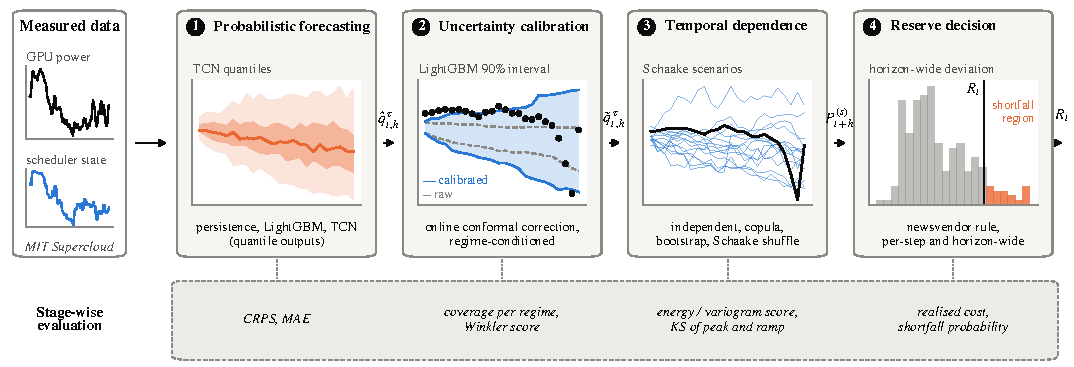
\includegraphics{figures/fig1_framework.pdf}
  \caption{Grid-oriented evaluation framework. Mini-plots show each stage's output for the test
  origin 2021-08-02 11:00 UTC (1-h resolution, 24-h horizon). Each stage passes its output to the
  next and is scored with its own metrics (bottom). Any component in a stage can be replaced
  without changing the other stages.}
  \label{fig:framework}
\end{figure*}

This paper addresses this gap with a public benchmark built from measured AI-cluster telemetry
and a stage-wise evaluation that follows a forecast from its quantiles to a reserve decision.
The study uses GPU telemetry and scheduler logs of the MIT Supercloud TX-Gaia cluster
\cite{samsi2021supercloud}. The main contributions are:
\begin{enumerate}
\item An open benchmark for grid-oriented probabilistic forecasting of AI-cluster GPU power.
From 100-ms telemetry of about 98{,}000 GPU jobs we construct a cluster-level series at 1-min
resolution, define three operational tasks (5-min/1-h, 15-min/4-h and 1-h/24-h) with
chronological splits that keep every target window inside its split, and score forecasts on
ramps, peaks and reserve cost in addition to CRPS and coverage.
\item Evidence that calibration under workload regime shifts depends on the forecaster, and a
model-agnostic correction. After a capacity increase, quantile LightGBM covers 63.4\% of
outcomes with a nominal 90\% interval at the 24-h horizon. A causal, regime-conditioned online
conformal correction raises coverage to 87.3\% and to at least 82.2\% in every workload regime.
A quantile TCN reaches 87.6\% without the correction, which then widens its intervals and raises
its CRPS from 1.462 to 1.535~kW.
\item A demonstration that calibrated per-step quantiles are not sufficient for a reserve held
over the horizon. Independent sampling of the steps distorts ramp and peak distributions and
over-procures reserve. Reordering the samples with past error trajectories (Schaake shuffle)
lowers the reserve cost by 7.6--10.6\% and keeps the shortfall rate close to its target.
\end{enumerate}

Section~II describes the data and tasks, Section~III the four-stage framework, Section~IV the
results, and Section~V concludes.

% =====================================================================
\section{Data and Benchmark Tasks}

\subsection{Cluster Telemetry}
TX-Gaia is a production AI cluster with 224 nodes, each with two NVIDIA V100 GPUs
\cite{samsi2021supercloud}. The public MIT Supercloud dataset records, for every GPU job, the
power draw of each assigned GPU every 100~ms through \texttt{nvidia-smi}, together with the
Slurm scheduler log (submission, start and end times and allocated resources). The records span
5~Feb. to 1~Oct.~2021. The dataset is released under the CC BY-NC-ND~4.0 license. We therefore
release code that rebuilds every series from the public source, not the processed data.

\subsection{Target Series}
For each job and node, we average the power of each GPU over 1-min intervals and sum over the
GPUs; summing over all jobs gives the measured GPU power of the cluster. GPUs not assigned to
any job draw idle power that the telemetry does not record. We add an assumed 40~W for each such
GPU, which sets a floor of about 18~kW when the cluster is empty. The target is therefore cluster
GPU IT power; CPU, cooling and facility losses are not included.

The GPU timestamps record US Eastern wall-clock time. The scheduler records UTC. Matching
job start and end times shows an offset of 5~h before 14~Mar.~2021 and 4~h after, and we convert
all telemetry to UTC. After this correction, the number of GPUs with telemetry equals the number
allocated by the scheduler at the median minute, and is at least 86\% of it in 90\% of minutes.
The resulting series has a mean of 31.2~kW, a 1-min maximum of 66.1~kW, and a largest 5-min
change of 28.3~kW.

Fig.~\ref{fig:data} shows the hourly series and the allocated GPUs. Two features matter for the
benchmark. The cluster empties for about a day every two to five weeks, consistent with scheduled
maintenance. In mid-May the weekly mean of allocated GPUs rises from about 250 to about 350. The training data thus span two
utilization levels, and the test period lies entirely in the second.

\begin{figure}[!t]
  \centering
  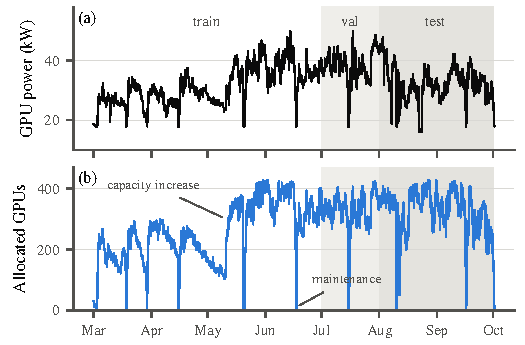
\includegraphics{figures/fig2_data.pdf}
  \caption{MIT Supercloud TX-Gaia cluster, March--September 2021, hourly means.
  (a) GPU IT power, including an assumed 40~W idle draw for unallocated GPUs.
  (b) GPUs allocated by the scheduler. Shading marks the training, validation and test periods.}
  \label{fig:data}
\end{figure}

\subsection{Tasks, Splits and Workload Regimes}
Three tasks cover intra-hour to day-ahead use: 5-min resolution with a 1-h horizon ($H=12$),
15-min resolution with a 4-h horizon ($H=16$), and 1-h resolution with a 24-h horizon ($H=24$).
A forecast is issued at every step. The splits are chronological: training from 1~Mar. to
30~Jun., validation in July, and test from 1~Aug. to 30~Sep.~2021. An origin belongs to a split
only if its whole target window lies in that split, so no target is shared across splits. The
test period contains 17{,}556, 5{,}840 and 1{,}440 origins for the three tasks.

Each origin is assigned one of four workload regimes from information available at that time.
\emph{Low} marks origins with fewer than 25\% of the GPUs allocated, which are mostly
maintenance windows. Other origins are labeled \emph{calm}, \emph{active} or \emph{volatile} by
terciles of the mean absolute power change over the preceding hour, with thresholds fitted on the
training period; an origin with more than 448 GPUs requested in the queue is labeled volatile.
In the test period the four regimes cover about 3\%, 17\%, 30\% and 50\% of the origins.

% =====================================================================
\section{Grid-Oriented Evaluation Framework}

Fig.~\ref{fig:framework} shows the framework. Each stage receives the output of the previous one,
passes its own output on, and is scored with its own metrics. Any component in a stage can be
replaced, so a new forecaster or scenario generator can be evaluated without changing the other
stages.


\subsection{Stage 1: Probabilistic Forecasting}
At origin $t$, a forecaster returns the quantiles $\hat q^{\,\tau}_{t,h}$ of the power
$P_{t+h}$ for $h=1,\dots,H$ and the nine levels
$\tau\in\{0.025,0.05,0.1,0.25,0.5,0.75,0.9,0.95,0.975\}$. Models are trained with the pinball
loss
\begin{equation}
\rho_\tau(u)=u\,\bigl(\tau-\mathbb 1\{u<0\}\bigr),\qquad u=P_{t+h}-\hat q^{\,\tau}_{t,h},
\end{equation}
whose mean over levels approximates half the CRPS \cite{koenker1978,gneiting2007}.
We evaluate four forecasters of increasing capacity.
\emph{Persistence} repeats the last value and adds the empirical quantiles of its training
errors at each horizon. \emph{Seasonal naive} repeats the value of the previous day in the same
way. \emph{LightGBM} \cite{ke2017lightgbm} fits one gradient-boosted model per quantile level,
with the horizon as an input, to the change from the value at the origin. Its inputs are
expressed relative to the current state: recent changes, rolling means and spreads, the
allocated and queued GPUs as fractions of the cluster, power per allocated GPU, and the hour
and weekday. The \emph{TCN} \cite{bai2018tcn} reads the same inputs over a 24-h lookback through
seven residual blocks of dilated causal convolutions (kernel 3, 64 channels, dilations 1 to 64)
and outputs all $H\times9$ quantiles of the change from the origin value. It is trained with the
pinball loss and stopped early on the validation loss; results are averaged over three seeds.

\subsection{Stage 2: Online Regime-Conditioned Calibration}
A forecaster fitted on one utilization level can be miscalibrated on another, as Section~IV-B shows for LightGBM. The calibrator
shifts each quantile by an empirical quantile of recent errors. With the score
$s^{\tau}_{j,h}=P_{j+h}-\hat q^{\,\tau}_{j,h}$, the calibrated quantile is
\begin{equation}
\tilde q^{\,\tau}_{t,h}=\hat q^{\,\tau}_{t,h}+\mathrm Q_\tau\bigl\{s^{\tau}_{j,h}:j\in
\mathcal C_{t,h}\bigr\},
\end{equation}
\begin{equation}
\mathcal C_{t,h}=\{\,j:\ j+h\le t,\ t-j\le W,\ r_j=r_t\,\},
\end{equation}
where $\mathrm Q_\tau$ is the empirical $\tau$-quantile, $W$ is a 14-day window and $r_t$ is the
workload regime. The condition $j+h\le t$ admits only origins whose targets are already observed,
so the correction uses no future information. If a regime has fewer than 200 scores in the
window, the regime condition is dropped. The calibration set starts with the validation period
and grows through the test period; corrections are refreshed every hour. This is a one-sided
form of conformalized quantile regression \cite{romano2019cqr} applied online
\cite{gibbs2021aci}. Stage-2 metrics are the empirical coverage of the central 90\% interval,
overall and per regime, and the Winkler interval score.

\subsection{Stage 3: Recovery of Temporal Dependence}
Quantiles at each step do not define a joint distribution over the horizon. Ramps, peak duration
and energy depend on how errors at consecutive steps move together. A scenario generator turns
the quantiles into $S=200$ trajectories $P^{(s)}_{t+1:t+H}$. We compare four generators.
\emph{Independent} sampling draws each step separately from the interpolated quantile function
$\tilde F^{-1}_{t,h}$. The \emph{Gaussian copula} \cite{pinson2009copula} draws correlated normal
variables with a horizon-by-horizon correlation estimated from validation errors. The
\emph{residual bootstrap} adds whole past error trajectories
$e_j=P_{j+1:j+H}-\hat q^{\,0.5}_{j,1:H}$, taken from origins observed by $t$, to the median
forecast. The \emph{Schaake shuffle} \cite{clark2004schaake} keeps the conditional marginals and
borrows only the rank structure of past errors. It draws $x_{h,(s)}=\tilde F^{-1}_{t,h}
\bigl((s-\tfrac12)/S\bigr)$ at each step, selects $S$ past error trajectories, and assigns to
scenario $s$ at step $h$ the sample whose rank equals the rank of $e_{j_s,h}$ among the selected
errors at that step.

Stage-3 metrics are the energy score (ES) \cite{gneiting2008es} and the variogram score (VS) of
order 0.5 \cite{scheuerer2015vs}, which reward correct dependence across steps, and grid
statistics of each trajectory: peak, largest ramp-up and ramp-down, energy, and duration above
the 90th percentile of validation power. For each statistic we compute the probability integral
transform (PIT) of the observed value within the scenario distribution. A generator that matches
the statistic gives uniform PIT values; we report the Kolmogorov--Smirnov (KS) distance from
uniform.

\subsection{Stage 4: Reserve Decision}
The scheduled power is the median forecast $\hat P_{t+h}=\tilde q^{\,0.5}_{t,h}$, and a reserve
$R_t$ covers positive deviations held over the whole horizon. With reserve cost $c_R$ per kW and
shortfall cost $c_S$ per kW, the realized cost is
\begin{equation}
c_R R_t + c_S\bigl(D_t-R_t\bigr)^{+},\qquad D_t=\max_{h}\bigl(P_{t+h}-\hat P_{t+h}\bigr).
\end{equation}
The expected cost is minimized by the $(1-c_R/c_S)$-quantile of $D_t$ (the critical fractile of
the newsvendor problem), which we estimate from the scenarios as
$R_t=\mathrm Q_{1-c_R/c_S}\{\max_h(P^{(s)}_{t+h}-\hat P_{t+h})\}_{s=1}^S$. The maximum over the
horizon depends on the joint behavior of the steps, so this decision tests Stage 3 directly. We
set $c_S=1$ and $c_R/c_S\in\{0.05,0.1,0.2\}$; at $0.1$ the target shortfall rate is 10\%. Stage-4
metrics are the realized mean cost (in kW-equivalent units) and the shortfall rate.

% =====================================================================
\section{Results}

All results are on the test period. Stage-3 and Stage-4 results use 3000 randomly selected test
origins for the 5-min and 15-min tasks and all 1{,}440 origins for the 24-h task.

\subsection{Forecast Skill After the Regime Shift}
Table~\ref{tab:forecast} reports Stages 1 and 2. Seasonal naive is omitted: its CRPS of
2.23--2.30~kW is 1.5 to 5 times that of the TCN, which is consistent with the weak daily
periodicity of the cluster load in Fig.~\ref{fig:data}. Persistence is hard to beat on the median: it has the lowest mean
absolute error (MAE) at 5-min and 15-min resolution. The TCN has the lowest CRPS in all three
tasks, 0.438, 0.741 and 1.462~kW, with a standard deviation over seeds of at most 0.006~kW.
LightGBM improves on persistence in CRPS at 5-min resolution only, and at the 24-h horizon its
CRPS of 1.746~kW is higher than that of persistence (1.607~kW).

\begin{table}[!t]
  \centering
  \caption{Forecast skill and calibration on the test period (Aug.--Sep.\ 2021)}
  \label{tab:forecast}
  \footnotesize
  % BEGIN AUTO TABLE-I (generated by paper/make_tables.py; do not edit by hand)
\begin{tabular}{@{}lrrrrr@{}}
\toprule
Forecaster & CRPS & MAE & Cov. & Min cov. & Winkler \\
 & (kW) & (kW) & (\%) & (\%) & \\
\midrule
\multicolumn{6}{@{}l}{\emph{5-min / 1-h}} \\
Persistence & 0.504 & 0.738 & 82.9 & 68.0 & 8.01 \\
LightGBM & 0.481 & 0.792 & 82.4 & 73.1 & 7.07 \\
LightGBM + OC & 0.469 & 0.783 & 87.9 & 77.2 & 6.80 \\
TCN & \textbf{0.438} & 0.747 & 88.3 & 86.8 & 6.11 \\
TCN + OC & \textbf{0.438} & 0.746 & \textbf{88.4} & 87.3 & 6.13 \\
\addlinespace
\multicolumn{6}{@{}l}{\emph{15-min / 4-h}} \\
Persistence & 0.809 & 1.286 & 83.2 & 62.6 & 12.04 \\
LightGBM & 0.823 & 1.360 & 73.9 & 59.3 & 12.07 \\
LightGBM + OC & 0.769 & 1.328 & 87.9 & 71.3 & 10.81 \\
TCN & \textbf{0.741} & 1.313 & \textbf{88.5} & 84.4 & 9.98 \\
TCN + OC & 0.751 & 1.319 & 87.9 & 83.9 & 10.15 \\
\addlinespace
\multicolumn{6}{@{}l}{\emph{1-h / 24-h}} \\
Persistence & 1.607 & 2.801 & 85.7 & 50.7 & 21.95 \\
LightGBM & 1.746 & 2.844 & 63.4 & 57.3 & 25.91 \\
LightGBM + OC & 1.551 & 2.850 & 87.3 & 82.2 & 20.69 \\
TCN & \textbf{1.462} & 2.739 & 87.6 & 84.3 & 18.59 \\
TCN + OC & 1.535 & 2.841 & \textbf{87.8} & 83.1 & 20.17 \\
\bottomrule
\end{tabular}  % END AUTO TABLE-I
  \\[2pt]
  \parbox{\columnwidth}{\scriptsize OC: online regime-conditioned calibration. Cov.: empirical
  coverage of the central 90\% interval. Min cov.: lowest coverage over the four workload regimes.
  TCN rows: mean of three seeds. Bold: lowest CRPS and coverage closest to 90\% per task.}
\end{table}

\subsection{Calibration Under the Regime Shift}
Without correction, LightGBM covers 82.4\%, 73.9\% and 63.4\% of outcomes with its nominal
90\% interval in the three tasks. At the 24-h horizon its mean interval width is 5.4~kW, half the
10.9~kW of the TCN. Most of its training data come from the lower utilization level before
May, and narrow intervals on the fuller test-period cluster are consistent with quantiles learned
from the smaller swings of that level. The deficit is present in every regime (Fig.~\ref{fig:regime}), so it is a shift in
level rather than a problem confined to maintenance windows.

The online correction raises LightGBM coverage to 87.9\%, 87.9\% and 87.3\%, and the lowest
regime coverage at the 24-h horizon from 57.3\% to 82.2\%. CRPS falls from 1.746 to 1.551~kW
and the Winkler score from 25.91 to 20.69. The remaining deficit of 2--3 points is consistent with
the lag of a 14-day window behind changes in the error distribution. The
regime condition mainly evens out coverage across regimes: at 5-min resolution, the calm,
active and volatile regimes reach 88.4\%, 88.4\% and 88.0\%.

The TCN covers 88.3\%, 88.5\% and 87.6\% without correction, and at least 84.3\% in every
regime. Its 24-h lookback includes the current utilization level and recent volatility,
which is consistent with interval widths that adapt at the origin. Applied to the TCN, the correction changes coverage by less
than one point and widens the 24-h interval from 10.9 to 12.6~kW, which raises CRPS from 1.462 to
1.535~kW. The correction is therefore a safety net with a small cost. It recovers most of the
coverage lost by a forecaster that does not track the regime, and it adds width to one that
already does.

\begin{figure}[!t]
  \centering
  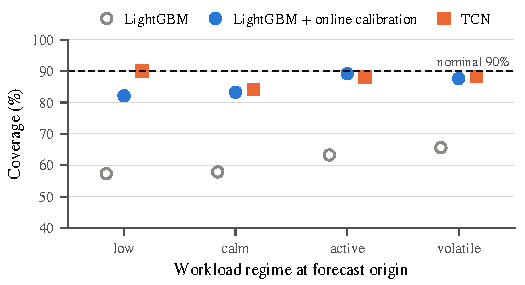
\includegraphics{figures/fig3_regime_coverage.pdf}
  \caption{Empirical coverage of the central 90\% interval by workload regime at the forecast
  origin, 1-h resolution, 24-h horizon, test period. TCN: mean of three seeds.}
  \label{fig:regime}
\end{figure}

\begin{figure*}[!t]
  \centering
  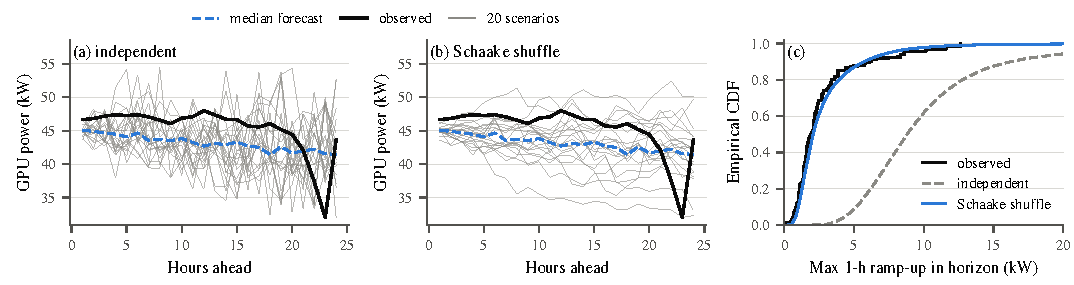
\includegraphics{figures/fig4_scenarios.pdf}
  \caption{Scenarios from the quantile TCN, 1-h resolution, 24-h horizon.
  (a), (b) Twenty scenarios for the test origin 2021-08-02 11:00 UTC, selected as the largest
  observed 1-h ramp-up among origins outside the low-load regime whose observed window stays above 20~kW.
  (c) Empirical CDF of the maximum 1-h ramp-up within the horizon over all 1440 test origins.}
  \label{fig:scenarios}
\end{figure*}

\subsection{Temporal Structure of the Scenarios}
Table~\ref{tab:scenarios} reports Stages 3 and 4 for the TCN quantiles. Independent sampling has
the largest ES and VS in every task, and its KS distances for the peak (0.52--0.66) and the
largest ramp-up (0.70--0.88) show that the observed statistics are concentrated at one end of
the simulated distribution. Consecutive forecast errors of the cluster load are positively correlated.
Sampling the steps separately removes this correlation, so simulated trajectories move up and
down from step to step far more than the observed load (Fig.~\ref{fig:scenarios}a, c).

All three generators that restore dependence reduce these distances. The Gaussian copula fixes
most of the peak distribution (KS 0.14--0.16) but leaves ramps biased (0.35--0.42). This is consistent with a Gaussian dependence
structure, estimated once on July, that does not match the shape of the step-to-step changes. The residual bootstrap reproduces ramps and peaks at 5-min and 15-min resolution, but
it ignores the forecaster's conditional spread: it adds the same pool of past errors to every
origin. The Schaake shuffle combines the conditional marginals of the TCN with the empirical
rank structure. It has the lowest ES and VS in all three tasks and KS distances of 0.07--0.13 for
ramp-up and 0.08--0.09 for the peak.

\begin{table}[!t]
  \centering
  \caption{Scenario quality and horizon-wide reserve, quantile TCN, test period}
  \label{tab:scenarios}
  \footnotesize
  \setlength{\tabcolsep}{4pt}
  % BEGIN AUTO TABLE-II (generated by paper/make_tables.py; do not edit by hand)
\begin{tabular}{@{}lrrrrrr@{}}
\toprule
Generator & ES & VS & KS & KS & Reserve & Short- \\
 & & & peak & ramp & cost & fall (\%) \\
\midrule
\multicolumn{7}{@{}l}{\emph{5-min / 1-h}} \\
Independent & 2.38 & 17.7 & 0.52 & 0.70 & 0.353 & 4.7 \\
Gaussian copula & \textbf{2.30} & 13.0 & 0.14 & 0.35 & 0.333 & 7.1 \\
Residual bootstrap & 2.43 & 13.7 & \textbf{0.06} & \textbf{0.07} & 0.390 & 11.0 \\
Schaake shuffle & \textbf{2.30} & \textbf{12.5} & 0.08 & \textbf{0.07} & \textbf{0.326} & \textbf{10.5} \\
\addlinespace
\multicolumn{7}{@{}l}{\emph{15-min / 4-h}} \\
Independent & 4.83 & 60.5 & 0.62 & 0.81 & 0.668 & 4.2 \\
Gaussian copula & 4.61 & 38.5 & 0.16 & 0.38 & 0.621 & 7.3 \\
Residual bootstrap & 4.75 & 37.4 & \textbf{0.07} & \textbf{0.12} & 0.714 & \textbf{10.2} \\
Schaake shuffle & \textbf{4.58} & \textbf{36.5} & 0.09 & 0.13 & \textbf{0.607} & 9.3 \\
\addlinespace
\multicolumn{7}{@{}l}{\emph{1-h / 24-h}} \\
Independent & 12.23 & 250.5 & 0.66 & 0.88 & 1.002 & 3.3 \\
Gaussian copula & 11.78 & 163.0 & 0.16 & 0.42 & 0.935 & 5.2 \\
Residual bootstrap & 12.16 & 159.7 & 0.17 & 0.12 & 1.026 & \textbf{7.6} \\
Schaake shuffle & \textbf{11.75} & \textbf{156.6} & \textbf{0.09} & \textbf{0.09} & \textbf{0.896} & \textbf{7.6} \\
\bottomrule
\end{tabular}  % END AUTO TABLE-II
  \\[2pt]
  \parbox{\columnwidth}{\scriptsize ES: energy score; VS: variogram score; KS: Kolmogorov--Smirnov
  distance of the PIT of the observed statistic from uniform. Reserve held over the whole horizon,
  $c_R/c_S = 0.1$ (target shortfall 10\%). 200 scenarios per origin; 3000 test origins (1440 for
  the 24-h task).
  Bold: best per task; for shortfall, closest to 10\%.}
\end{table}


\subsection{Effect on the Reserve Decision}
The distortion carries into the reserve held over the horizon. With independent scenarios,
the simulated trajectories contain larger excursions than the observed load, so the estimated
quantile of $D_t$ is too high. At $c_R/c_S=0.1$, the reserve is 9.43~kW at the 24-h horizon and the realized
shortfall rate is 3.3\% against a 10\% target. The Schaake shuffle sets a reserve of 7.59~kW
with a shortfall rate of 7.6\%, and its mean cost is 0.896 against 1.002. Across the three tasks
the cost falls by 7.6\%, 9.1\% and 10.6\%, and the shortfall rate is 10.5\%, 9.3\% and 7.6\%.
The Schaake shuffle also has the lower cost at $c_R/c_S=0.05$ and $0.2$ in every task; at
$0.2$ the reduction is 15.5--17.8\%.

The residual bootstrap shows why the stages must be evaluated together. At 5-min resolution it
matches ramps as well as the Schaake shuffle (KS 0.07) yet costs 0.390 against 0.326, because its
reserve barely changes with the forecast spread at each origin. Correct temporal structure and
correct conditional spread are both needed before a forecast gives a good reserve.

% =====================================================================
\section{Conclusion}

This paper built an open benchmark from measured GPU telemetry of a 448-GPU AI cluster and
evaluated probabilistic forecasts through four stages that end in a reserve decision. The
stage-wise evaluation locates where forecast value is lost. After a capacity increase, a quantile
LightGBM model covered 63.4\% of outcomes with a nominal 90\% interval at the 24-h horizon; a
causal online conformal correction restored 87.3\%, while a quantile TCN was close to nominal
without it. At the next stage, calibrated quantiles sampled step by step distorted ramps and
peaks and over-procured reserve held over the horizon. Reordering the samples with past error
trajectories kept the conditional spread, matched ramp and peak statistics, and lowered the
reserve cost by 7.6--10.6\% at a 10\% target shortfall rate.

The results describe one cluster in 2021 and its GPU IT power, with an assumed idle draw for
unallocated GPUs. Facility-level forecasts need cooling and power-conversion models on top of
this target, and the benchmark can be extended to other measured workloads, such as recent
generative-AI power profiles \cite{vercellino2026nlr}. Formal tests of the differences between
methods and a sensitivity study of the idle-power assumption are the next steps.

\section*{Code Availability}
The processing, baseline and evaluation code (DCGridBench) is available at
\url{https://github.com/dinglin613/Data_center_forecasting}.

% =====================================================================
\bibliographystyle{IEEEtran}
\bibliography{references}

\end{document}
